%!TEX program = xelatex
\documentclass{article}

\usepackage[dvipsnames]{xcolor}

\usepackage{fancyhdr}
\usepackage{extramarks}
\usepackage{amsmath}
\usepackage{amsthm}
\usepackage{amsfonts}
\usepackage{tikz}
\usepackage[plain]{algorithm}
\usepackage{algpseudocode}

\usepackage{ctex}
\usepackage{indentfirst}
\usetikzlibrary{automata,positioning,shapes.geometric,arrows.meta,patterns,calc}

%
% Basic Document Settings
%

\topmargin=-0.45in
\evensidemargin=0in
\oddsidemargin=0in
\textwidth=6.5in
\textheight=9.0in
\headsep=0.25in

\linespread{1.1}

\pagestyle{fancy}
\lhead{\hmwkAuthorName}
\chead{\hmwkClass\ (\hmwkClassInstructor): \hmwkTitle}
\rhead{\firstxmark}
\lfoot{\lastxmark}
\cfoot{\thepage}

\renewcommand\headrulewidth{0.4pt}
\renewcommand\footrulewidth{0.4pt}

\setlength\parindent{0pt}


\setlength{\parindent}{2em}  % 2em代表首行缩进两个字符

%
% Create Problem Sections
%

\newcommand{\enterProblemHeader}[1]{
    \nobreak\extramarks{}{Problem \arabic{#1} continued on next page\ldots}\nobreak{}
    \nobreak\extramarks{Problem \arabic{#1} (continued)}{Problem \arabic{#1} continued on next page\ldots}\nobreak{}
}

\newcommand{\exitProblemHeader}[1]{
    \nobreak\extramarks{Problem \arabic{#1} (continued)}{Problem \arabic{#1} continued on next page\ldots}\nobreak{}
    \stepcounter{#1}
    \nobreak\extramarks{Problem \arabic{#1}}{}\nobreak{}
}

\setcounter{secnumdepth}{0}
\newcounter{partCounter}
\newcounter{homeworkProblemCounter}
\setcounter{homeworkProblemCounter}{1}
\nobreak\extramarks{Problem \arabic{homeworkProblemCounter}}{}\nobreak{}

%
% Homework Problem Environment
%
% This environment takes an optional argument. When given, it will adjust the
% problem counter. This is useful for when the problems given for your
% assignment aren't sequential. See the last 3 problems of this template for an
% example.
%
\newenvironment{homeworkProblem}[1][-1]{
    \ifnum#1>0
        \setcounter{homeworkProblemCounter}{#1}
    \fi
    \section{Problem \arabic{homeworkProblemCounter}}
    \setcounter{partCounter}{1}
    \enterProblemHeader{homeworkProblemCounter}
}{
    \exitProblemHeader{homeworkProblemCounter}
}

%
% Homework Details
%   - Title
%   - Due date
%   - Class
%   - Section/Time
%   - Instructor
%   - Author
%

\newcommand{\hmwkTitle}{The Kinematics of Mass Points}
\newcommand{\hmwkDueDate}{\today}
\newcommand{\hmwkClass}{University Physics}
\newcommand{\hmwkClassTime}{}
\newcommand{\hmwkClassInstructor}{WHU}
\newcommand{\hmwkAuthorName}{\textbf{Lai Wei}}

%
% Title Page
%

\title{
    \vspace{2in}
    \textmd{\textbf{\hmwkClass:\ \hmwkTitle}}\\
    \normalsize\vspace{0.1in}\small{Date: \hmwkDueDate}\\
    \vspace{0.1in}\large{\textit{\hmwkClassInstructor}}
    \vspace{3in}
}

\author{\hmwkAuthorName}
\date{}

\renewcommand{\part}[1]{\textbf{\large Part \Alph{partCounter}}\stepcounter{partCounter}\\}

%
% Various Helper Commands
%

% Useful for algorithms
\newcommand{\alg}[1]{\textsc{\bfseries \footnotesize #1}}

% % For derivatives
% \newcommand{\deriv}[1]{\frac{\mathrm{d}}{\mathrm{d}x} (#1)}

% For partial derivatives
\newcommand{\pderiv}[2]{\frac{\partial}{\partial #1} (#2)}

% Integral dx
\newcommand{\dx}{\mathrm{d}x}

% Alias for the Solution section header
\newcommand{\solution}{\textbf{\large Solution}}

% Probability commands: Expectation, Variance, Covariance, Bias
\newcommand{\E}{\mathrm{E}}
\newcommand{\Var}{\mathrm{Var}}
\newcommand{\Cov}{\mathrm{Cov}}
\newcommand{\Bias}{\mathrm{Bias}}

% 我的newcommand
\newcommand{\degree}{^{\circ}}
\newcommand{\arrow}{-{Stealth[length=4mm,width=2mm]}}
\newcommand{\rmd}{\mathrm{d}}
\newcommand{\deriv}[2]{\frac{\rmd #1}{\rmd #2}}

\begin{document}

\maketitle

\pagebreak

\begin{homeworkProblem}
    在离水面高为\(h\)的岸上,有人用绳拉船靠岸,如图所示。设人以匀速率\(v_{0}\)收绳,试求:
    当船距岸边\(x_{0}\)时,船的速度和加速度的大小各是多少?

    \[
        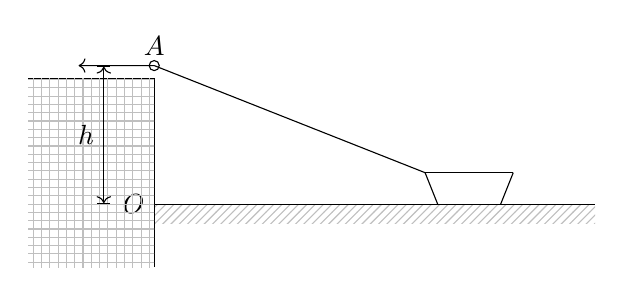
\begin{tikzpicture}[scale=0.8]
        \coordinate[label=left:$O$] (O) at (0,0);
        \coordinate[label=above:$A$] (A) at (0,2.2);
        \fill[pattern=north east lines, pattern color=gray!50] (0,0) rectangle (7,-0.3);
        \draw (0,-1) -- (0,2);
        \draw (O) -- (7,0);
        \draw (0,2) -- (-2,2);
        \fill[pattern=grid, pattern color=gray!50] (0,-1) rectangle (-2,2);
        \draw (A) circle (0.08);
        % 小船
        \draw (4.5,0) -- (5.5,0);
        \draw (4.5,0) -- (4.3,0.5);
        \draw (5.5,0) -- (5.7,0.5);
        \draw (4.3,0.5) -- (5.7,0.5);
        % 绳子
        \draw (A) -- (4.3,0.5);
        \draw[->] (A) -- (-1.2,2.2);
        % 尺寸标注
        \draw[|<->|] (-0.8,0) -- (-0.8,2.2) node[midway, left] {$h$};
        % \draw[|<->|] (0,-1) -- (5,-1) node[midway, below] {$x$};
        % \draw[dashed] (5,-1) -- (5,0);
        \end{tikzpicture}
    \]
    \\

    \textbf{Solution}
    \\

    \textbf{Part One}

    建立如图所示的坐标系。

    \[
        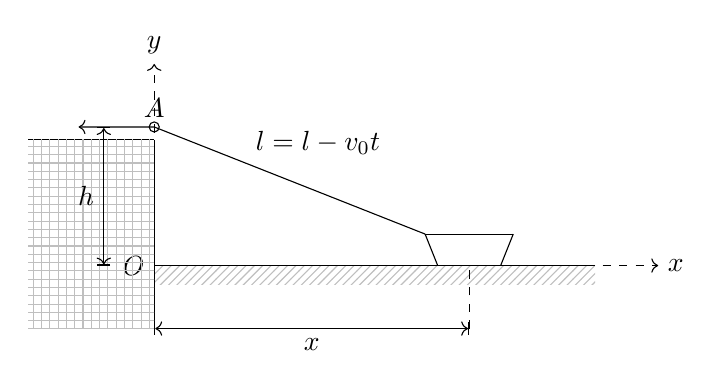
\begin{tikzpicture}[scale=0.8]
        \coordinate[label=left:$O$] (O) at (0,0);
        \coordinate[label=above:$A$] (A) at (0,2.2);
        \fill[pattern=north east lines, pattern color=gray!50] (0,0) rectangle (7,-0.3);
        \draw (0,-1) -- (0,2);
        \draw (O) -- (7,0);
        \draw (0,2) -- (-2,2);
        \fill[pattern=grid, pattern color=gray!50] (0,-1) rectangle (-2,2);
        \draw (A) circle (0.08);
        % 小船
        \draw (4.5,0) -- (5.5,0);
        \draw (4.5,0) -- (4.3,0.5);
        \draw (5.5,0) -- (5.7,0.5);
        \draw (4.3,0.5) -- (5.7,0.5);
        % 绳子
        \draw (A) -- (4.3,0.5);
        \draw[->] (A) -- (-1.2,2.2);
        \coordinate[label={above:$ l = l - v_{0}t $}] (rope) at (2.6,1.6);
        % 尺寸标注
        \draw[|<->|] (-0.8,0) -- (-0.8,2.2) node[midway, left] {$h$};
        \draw[|<->|] (0,-1) -- (5,-1) node[midway, below] {$x$};
        \draw[dashed] (5,-1) -- (5,0);
        % 坐标系
        \coordinate[label=right:$x$] (x) at (8,0);
        \coordinate[label=above:$y$] (y) at (0,3.2);
        \draw[->,dashed] (O) -- (x);
        \draw[->,dashed] (O) -- (y);
        \end{tikzpicture}
    \]

    设初始时刻,船与岸上\(A\)点之间的绳长为\(l_{0}\)。在任意时刻船离岸边的距离为\(x\),
    绳长为\(l_{0}\)。船在运动过程中,\(l\)和\(x\)均是时间\(t\)的函数。

    由题意,\(l = l - v_{0}t\),所以

    \[
    v_{0} = - \deriv{l}{t}
    \]

    又由几何关系

    \[
    l^{2} = x^{2} + h^{2}
    \]

    对上式两边同时对\(t\)求导,可得

    \[
    2 l \deriv{l}{t} = 2x \deriv{x}{t}
    \]

    则船的运动速度为

    \[
    v = \deriv{x}{t} = \frac{l}{x} \deriv{l}{t} = -\frac{l}{x} v_{0}
    \]
    \\

    \textbf{Part Two}

    再将速度对时间\(t\)求导,即可得到船的加速度为

    \[
    a = \deriv{v}{t} = - \frac{v_{0}}{x^{2}} \left(x \deriv{l}{t} - l \deriv{x}{t}\right)
    = -\frac{v_{0}^{2} h^{2}}{x^{3}}
    \]
    \\

    \textbf{Part Three}

    令\(x=x_{0}\),得船在离岸边为\(x_{0}\)时的速度和加速度分别为

    \[
    v = \frac{\sqrt{x_{0}^{2} + h^2}}{x_{0}} v_{0},\;
    a = -\frac{v_{0}^{2} h^{2}}{x^{3}}
    \]

\end{homeworkProblem}

\end{document}
